% modelo beamer
% http://latexbr.blogspot.com.br/
% aspectratio=169 - modo widescreen
\documentclass[aspectratio=169]{beamer}
\usepackage[utf8]{inputenc}
\usepackage[T1]{fontenc}
\usepackage[brazil]{babel}
\usepackage{graphics,amssymb,amsfonts,amsmath}
\usepackage{tikz}
\usepackage{enumerate,hyperref}
\usepackage{palatino}	% Fonte sem serifa
\usepackage{ragged2e}	% Paragrafo justificado
\usepackage{minted}	% Highlight para codigos de programacao
\usepackage{booktabs} % tabelas

% Tema, cor e fonte modo matematico
\usetheme{AnnArbor}
% \usetheme{Pittsburgh}
\usecolortheme{orchid}
\usefonttheme[onlymath]{serif}
% Veja mais temas e cores em http://www.hartwork.org/beamer-theme-matrix/

% Colocando numero de paginas no slide
\setbeamertemplate{footline}[frame number]

% Desativando os botoes de navegacao
\beamertemplatenavigationsymbolsempty

% Tela cheia
\hypersetup{pdfpagemode=FullScreen}

% Layout da pagina
\hypersetup{pdfpagelayout=SinglePage}

% Definicao de novos ambientes
\theoremstyle{Definition}
\newtheorem{defn}{Defini\c c\~ao}
\newtheorem{teo}[theorem]{Teorema}
\newtheorem{ex}[theorem]{Exemplo}

% Definicao de novos comandos
\providecommand{\sin}{} \renewcommand{\sin}{\hspace{2pt}\textrm{sen}}
\providecommand{\tan}{} \renewcommand{\tan}{\hspace{2pt}\textrm{tg}}
\newcommand{\R}{\mathbb{R}}

% Capa - requer o TikZ
\newcommand{\capa}{
  \begin{tikzpicture}[remember picture,overlay]
    \node at (current page.south west)
      {\begin{tikzpicture}[remember picture, overlay]
        \fill[shading=radial,top color=orange,bottom color=orange,middle color=yellow]
          (0,0) rectangle (\paperwidth,\paperheight);
      \end{tikzpicture}
      };
  \end{tikzpicture}
}

% Ambiente Java (minted)
\newminted{java}{bgcolor=cyan!10}

% Titulo
\title[\sc{Texto no rodap\'e}]{Modelo do Beamer - Digite o titulo}
\author[digite seu Nome]{digite seu Nome}
\institute{nome do instituto} % opcional
\date{\today}

\begin{document}
\justifying % Paragrafo justificado

% Primeiro frame: Capa
\begin{frame}
  \capa
  \titlepage
\end{frame}

\section{Introdu\c c\~ao}

% Frame 2: Introducao
\begin{frame}[fragile]\frametitle{Introdu\c c\~ao}
Este \'e um modelo do Beamer\cite{tantau2004user}, veja os c\'odigos e altere-os conforme sua necessidade.

Este exemplo cont\'em um pre\^ambulo e algumas figuras.

Este exemplo usa o pacote \verb|minted|. Para compilar \'e necess\'ario usar o comando\\
\verb|-shell-escape| pelo terminal.

\begin{minted}[bgcolor=lightgray!20]{bash}
pdflatex -shell-escape beamer_modelo2013.tex
ou
latexmk -pdf -shell-escape beamer_modelo2013.tex
\end{minted}

\vfill

\begin{flushright}
\url{latexbr.blogspot.com.br}\cite{LaTeXBR}
\end{flushright}

\end{frame}

% Imagem como plano de fundo
% Insere a imagem no proximo slide
{%
\usebackgroundtemplate{
  \centering
  
\includegraphics[width=\paperwidth]{fig/figBackground}
}

% Frame 3: plano de fundo
\begin{frame}
  \begin{center}
    % texto colorido
    \color{yellow}{\Huge Imagem como plano de fundo}
  \end{center}
\end{frame}
}
% esta chave 'fecha' a imagem,
% caso queira a figura em mais frames
% coloque os outros frames antes desta chave.

% Frame 4: expressoes matematicas
% a opcao fragile permite uso do verbatim
\begin{frame}[fragile]\frametitle{Express\~oes Matem\'aticas}

% Paragrafo
\setlength{\parindent}{2em}

Seja $f: \R \to \R$ tal que $y = \sin x$.

Este texto est\'a justificado\footnote{Nota de rodap\'e.} e com uma margem definida pelo comando

\begin{verbatim}
\setlength{\parindent}{2em}
\end{verbatim}

Exemplo de uma equa\c c\~ao matem\'atica centralizada.

\[
S = \int_a^b \frac{\sqrt x}{x}dx
\]
\end{frame}

% Frame 5: exemplo e solucao
\begin{frame}\frametitle{Exemplo e Solu\c c\~ao}
  
  \begin{block}{Exemplo}
    Este \'e um ambiente chamado \emph{block} com um titulo \emph{Exemplo}.\cite{knuth}\cite{lamport}
  \end{block}

  \begin{exampleblock}{Solu\c c\~ao}
    Este \'e um ambiente chamado \emph{exampleblock} com um titulo \emph{Solu\c c\~ao}.
  \end{exampleblock}

\end{frame}

% Frame 6: novos ambientes
\begin{frame}\frametitle{Novos ambientes}
  
  \begin{defn}
    Novo ambiente chamado \emph{defini\c c\~ao}.
  \end{defn}

  \begin{teo}
    Novo ambiente chamado \emph{teorema}.
  \end{teo}

\end{frame}

% Frame 7: verbatim
\begin{frame}[fragile]\frametitle{Verbatim}
Para usar o verbatim no Beamer \'e necess\'ario usar a op\c c\~ao \verb|fragile|.

\begin{verbatim}
 \begin{frame}[fragile]\frametitle{Verbatim}
  % qualquer codigo LaTeX ou outros
 \end{frame}
\end{verbatim}

\end{frame}

% Frame 8: Linguagem de programacao
\begin{frame}[fragile]\frametitle{Linguagem de programa\c c\~ao}
Para mostrar c\'odigos de linguagem de programa\c c\~ao use o pacote \verb|minted|.

Exemplo de c\'odigo Java.

\begin{javacode}
public class HelloWorldApp {
    public static void main (String args[])
    {
      System.out.println("Hello World!");
    }
}
\end{javacode}

Para compilar com o pacote \verb|minted| \'e necess\'ario usar o comando \verb|-shell-escape| pelo terminal.

\begin{minted}[bgcolor=lightgray!20]{bash}
pdflatex -shell-escape minted01.tex
ou
latexmk -pdf -shell-escape minted01.tex
\end{minted}
\end{frame}

% Frame 9: Inserindo figuras
\begin{frame}\frametitle{Inserindo figuras}
Figuras devem ser inseridas no formato PNG, JPG ou PDF.

  \begin{figure}[h]
    \centering
    \includegraphics[height=0.6\paperheight]{fig/figCoordEsf02}
    %\includegraphics[height=6cm]{figCoordEsf02}
    \caption{Sistema de coordenadas esf\'ericas.}\label{figCoordEsf02}
  \end{figure}
\end{frame}

% Frame 10: figuras TikZ
% \begin{frame}\frametitle{Figuras TikZ}
% Figuras feitas com TikZ.

%   \begin{figure}[h]
%     \centering
%     \input{figuras/integral}
%     \caption{Integral.}\label{figintegral}
%   \end{figure}
% \end{frame}

% Frame 11: tabela
\begin{frame}\frametitle{Tabelas}
  \begin{table}
    \centering
    \begin{tabular}{cclrr}
      \toprule
      ID & Quant & Produto & Unit & Total\\
      \midrule
      1 & 2 & manga     & 3,00 & 6,00\\
      2 & 7 & laranja   & 1,20 & 8,40\\
      3 & 5 & banana    & 3,50 & 17,50\\
      4 & 3 & melancia  & 8,00 & 24,00\\
      5 & 4 & abacaxi   & 4,00 & 16,00\\
      \midrule
       Total &   &           &  & 71,90\\
      \bottomrule
    \end{tabular}
    \caption{Lista de compras}
  \end{table}
\end{frame}


\section{Transi\c c\~ao}

% Frame 12: Transicao
\begin{frame}\frametitle{Transi\c c\~ao}
Um pequeno exemplo de transi\c c\~ao.

\pause

\begin{enumerate}[a)]
  \item<2-> primeiro;
  \item<3-> segundo;
  \item<4-> terceiro.
\end{enumerate}
\end{frame}

% Frame 13: Bibliografia
\begin{frame}\frametitle{Bibliografia}
  % estilo da bibliografia
  \bibliographystyle{abbrv}
  % chamando o arquivo refs.bib
  \bibliography{refs}
\end{frame}

% Veja mais temas e cores em http://www.hartwork.org/beamer-theme-matrix/
% http://latexbr.blogspot.com.br/

\end{document}
